\documentclass[12px]{scrartcl}

 
\usepackage{float}

\usepackage[utf8]{inputenc}

\usepackage[T1]{fontenc}

\usepackage{lmodern}

\usepackage[ngerman]{babel}

\usepackage{amsmath}

\usepackage{graphicx}


 

\title{Versuch AP2\\ Bestimmung des Planckschen Wirkungsquantums - Der Photoelektrische Effekt}

\author{Frederik Strothmann, Henrik Jürgens}

\date{\today}


\begin{document}


 %deckblatt erstellen

\maketitle
\newpage
\tableofcontents
\newpage

%einleitung zu dem experiment

\section{Einleitung}

In diesem Versuch wird eine Photozelle (mit Meßverstärker) mit verschiedenen Spektrallinien einer Quecksilberdampflampe beleuchtet, um einen Vergleich zwischen klassischer Theorie und Quantentheorie durchzuführen.
%1
Außerdem wird das Verhältnis $\frac{h}{e}$ und hieraus die Plancksche Konstante h
bestimmt.
%2
In ergänzenden Versuchsteilen können dann umgekehrt aus der Stoppspannung die Wellenlänge des Lichts verschiedenfarbiger Leuchtdioden bestimmt werden.
%3
Außerdem schätzen wir die Quantenausbeute der Photozelle und die Lichtleistung der Quecksilber-Spektrallinien
unter Verwendung einer Halbleiter-Photodiode ab.
%versuchsaufbau mit skizze

\section{Versuchsaufbau}
													
\begin{figure}[H]
\centering
    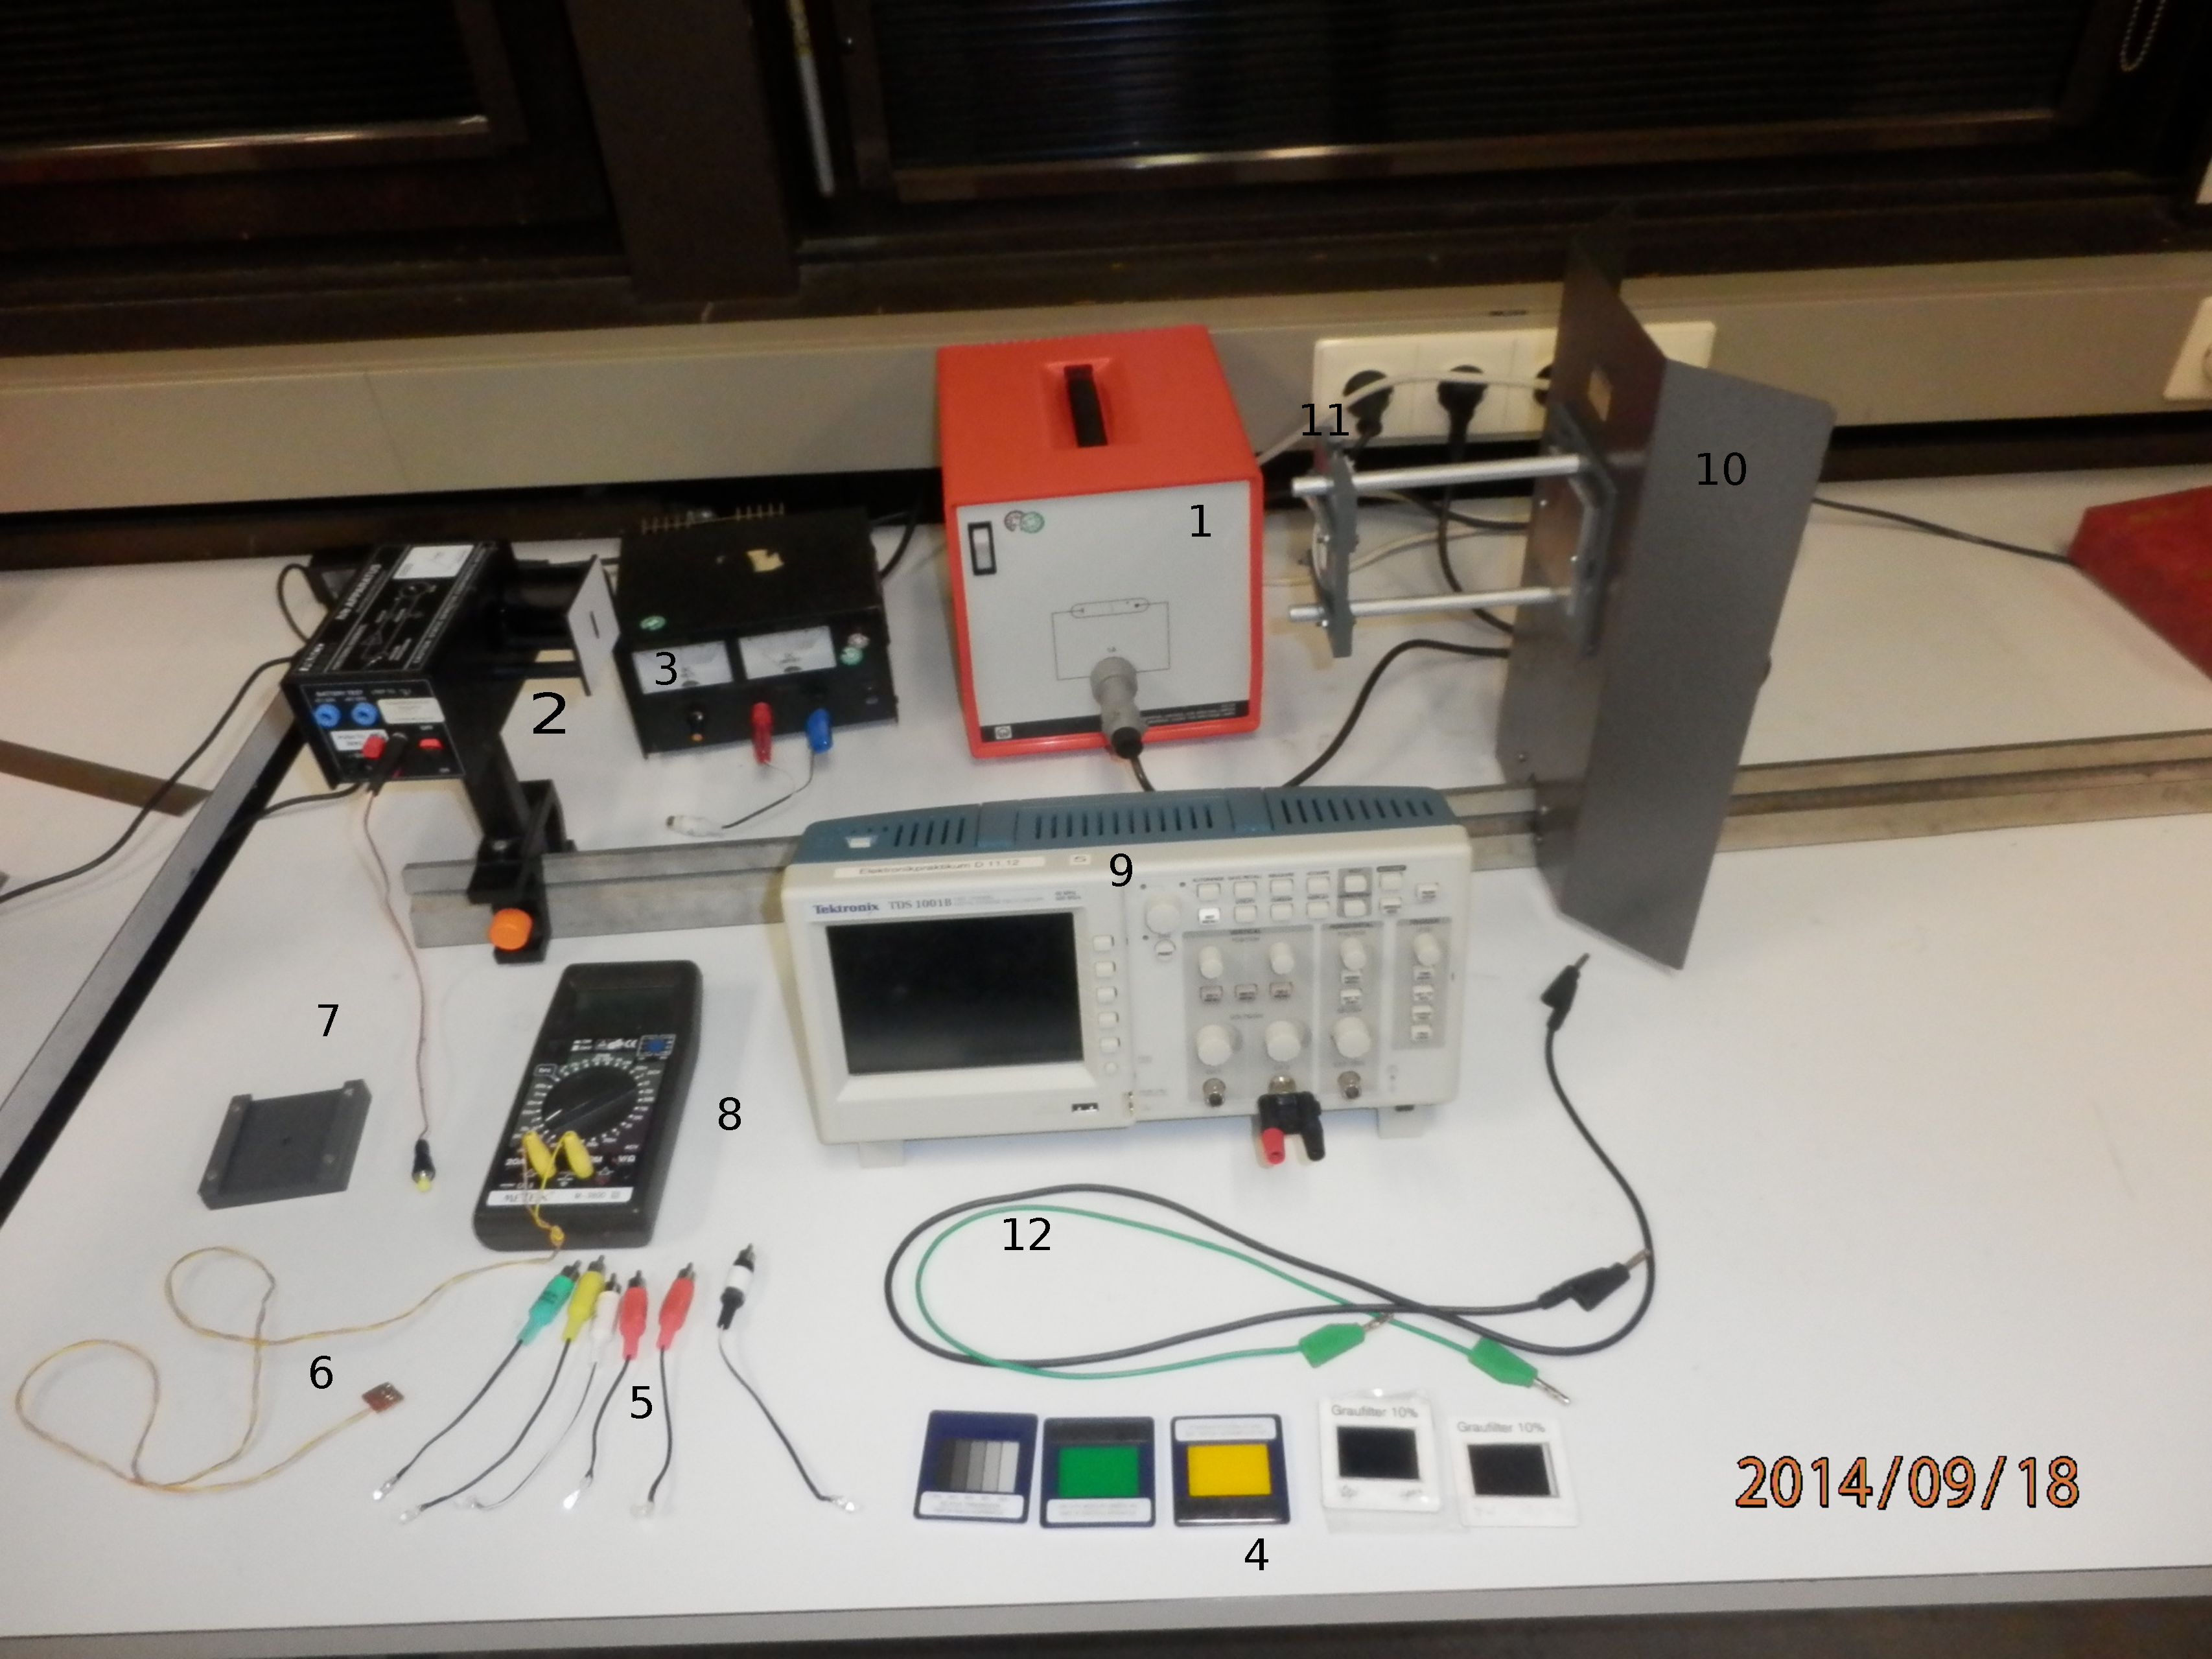
\includegraphics[scale = 0.2]{versuchsmaterialien.pdf}
  	\caption[Für den Versuch verwendete Materialien]{Für den Versuch verwendete Materialien}
  \label{fig:a_3_A}
\end{figure}

\begin{enumerate}
\item	Netzgerät für die Lampe

\item	h/e-Gerät

\item	Netzgerät für die Dioden (5)

\item	grün, gelb, 10\% und 20-100\% Filter

\item	rot, gelb, grün und blaue Dioden

\item	Photodiode

\item	Halterung für die Dioden

\item	DMM

\item	Oszilloskop

\item	Sichtschirm mit dahinter stehender Lampe

\item	Linsengitter Kombination

\item	Verbindungskabel
\end{enumerate}

Das Licht aus der Lampe wird durch die Filterlinsen Kombination in die Spektralfarben aufgespalten, sodass mit dem h/e-Gerät die Stoppspannung bestimmt werden kann.


\section{Vergleich zwischen Wellen- und Quantenmodell und Bestimmung der Planckschen
Konstante $h$}


\subsection{Praktische Durchführung}
Das Quantenmodell des Lichts besagt, dass die maximale Energie $E_{kin,max}$ von Photoelektronen nur von der Frequenz des einfallenden Lichtes abhängt und von der Lichtintensität unabhängig ist.
Dagegen sagt das klassische Wellenmodell des Lichtes voraus, dass die maximale Energie $E_{kin,max}$ der Photoelektronen von der Lichtintensität abhängt.
Entsprechend dem Quantenmodell des Lichts ist die Energie der Lichtquanten direkt proportional zu ihrer Frequenz: Je höher die Frequenz, desto mehr Energie hat das Quant. Beim Experimentieren wollen wir den Proportionalitätsfaktor, die Plancksche Konstante, bestimmen.
Wir werden dazu unterschiedliche Spektrallinien der Quecksilberdampflampe verwenden und die Maximalenergie $E_{kin,max}$ der Photoelektronen bzw die Stoppspannung $U_0$ ($U_0\cdot e = E_{kin,max}$) als Funktion der Wellenlänge und Frequenz untersuchen:
\begin{enumerate}
\newpage
\item Im (Gitter-)Spektrum der Quecksilberdampflampe sehen wir 5 Farben in mindestens 2 Ordnungen.
%Abbildung 5 aus der versuchsbeschreibung mit den ordnungen einfügen
\begin{figure}[htbp] 
  \centering
    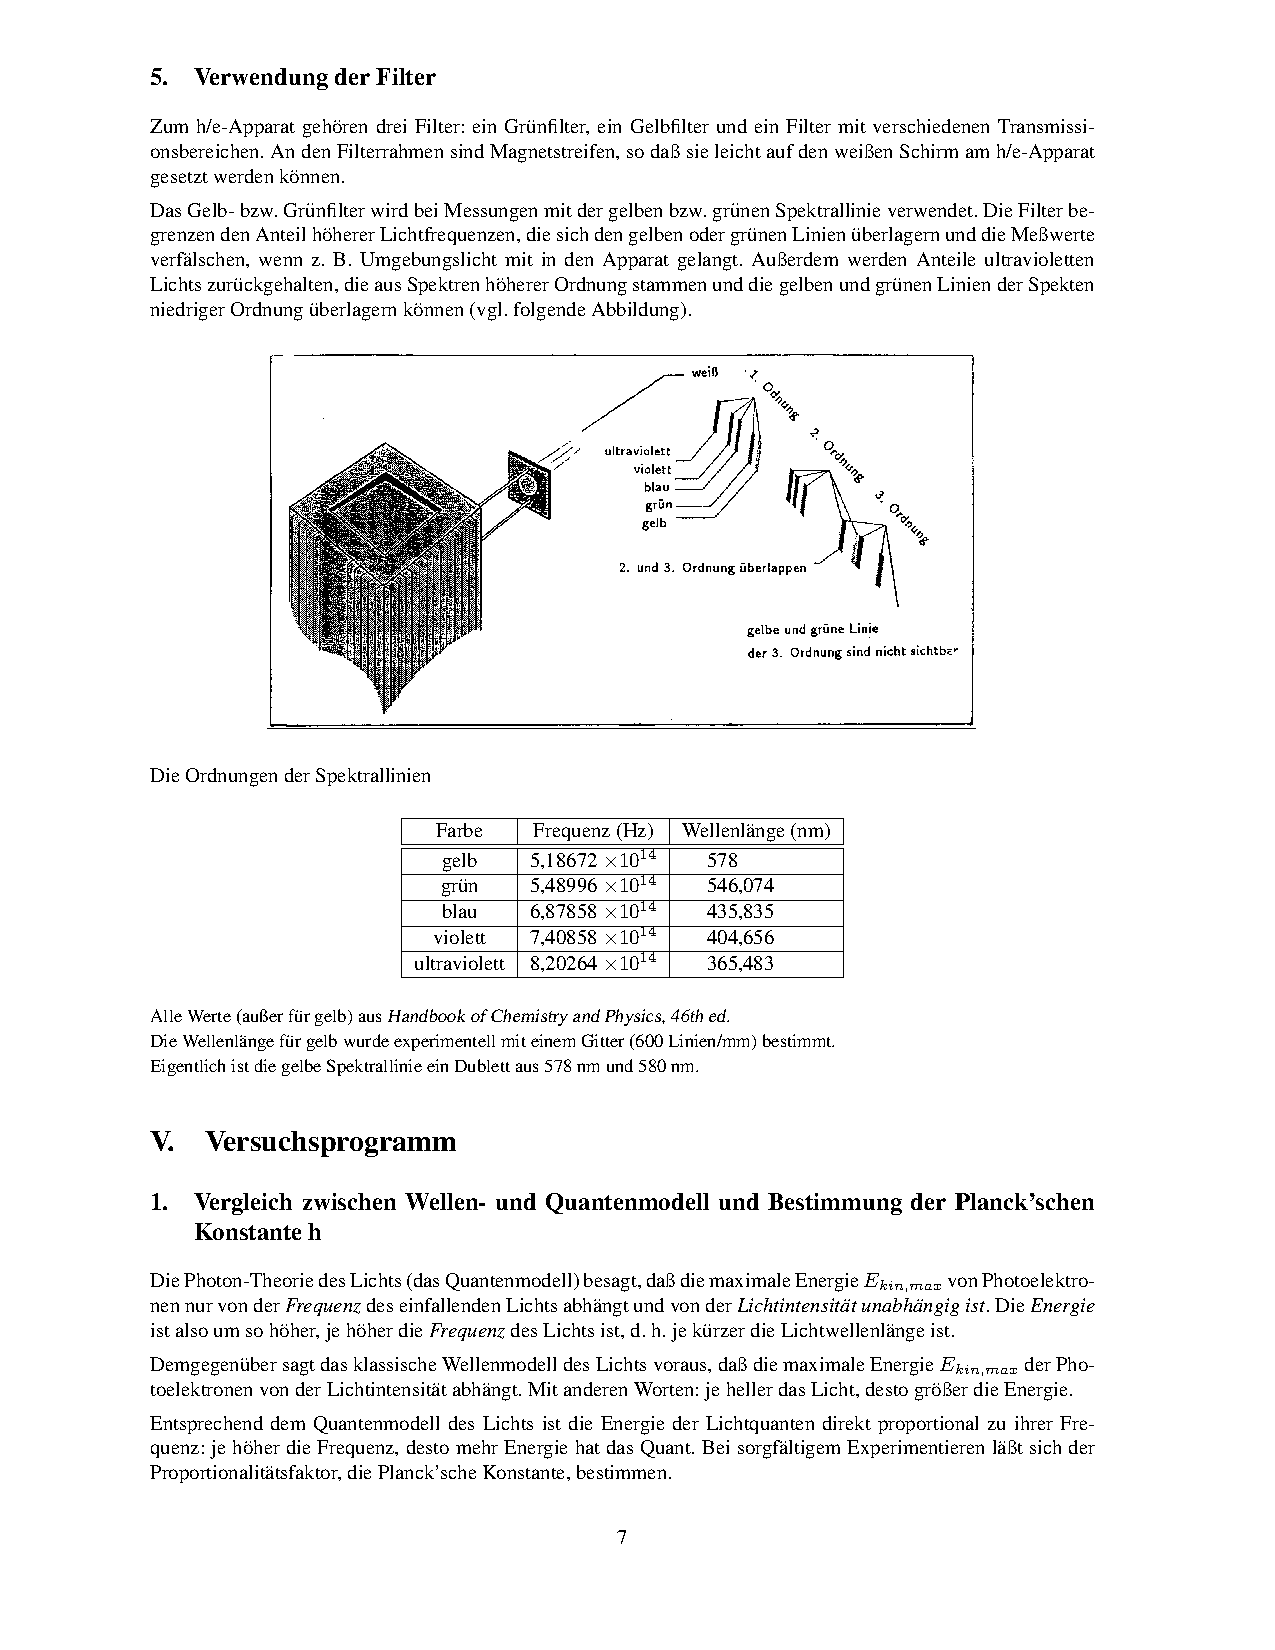
\includegraphics[trim = 35mm 150mm 1mm 60mm, clip, scale = 1]{abb5.pdf}
  	\caption[Skizze des durch die Linse beobachtbaren Lichtbeugungsmusters]{Skizze des durch die Linse beobachtbaren Lichtbeugungsmusters\footnotemark}
  \label{fig:schaltskizze}
\end{figure}
\footnotetext{Abbildung entnommen von http://www.atlas.uni-wuppertal.de/~kind/ap22ap2.pdff Seite 7 am 17.09.2014}
	
Wir stellen nun den h/e-Apparat so ein, dass nur eine Farbe aus dem Spektrum erster Ordung in die Öffnung der Photozelle fällt.
\item Wir messen für jede Farbe der ersten Ordnung die Stoppspannung mit dem Digitalvoltmeter und setzen den
Gelb- bzw. Grünfilter vor den weißen Schirm, falls wir die gelbe bzw. grüne Spektrallinie vermessen.
\item Danach wiederholen wir die Messung für die fünf Farben zweiter Ordnung.
\item Wir benutzen dann die Transmissionsfilter (Graufilter), um die Intensitätsabhängigkeit der Stoppspannung zu messen.
\end{enumerate}
\subsection{Verwendete Formeln}
\textbf{Verwendete Bezeichnungen:}
\begin{enumerate}
\item $U_0$ := Stoppspannung\\ (Kann über ein DMM am $\frac{h}{e}$-Gerät abgelesen werden, da dieses sich wie ein Kondensator verhält, sodass ab einer bestimmten Spannung keine weiteren Elektronen von der Anode aufgenommen werden können.)
\item $h$ := Plancksches Wirkungsquantum\\
(soll in diesem Versuch bestimmt werden)
\item $e$ := Elemetarladung
(Wird in diesem Versuch ohne Fehler angenommen wird, da dieser im Vergleich zu unserer Messung verschwindend gering ist. $e$= 1,602176...$\cdot10^{-19}C$)
\item $W_0$ := Auslösearbeit\\
(Wird benötigt wird, um die Elektronen von der Materialoberfläche zu lösen)
\item $Y_0$ := Y-Achsenabschnitt
\item $m$ := Steigung der Geraden

\end{enumerate}
\textbf{Nach der Einsteinschen Formel ergibt sich für die Stoppspannung die folgende Beziehung:}
\begin{align}
U_0 = \frac{h}{e}\nu + \frac{W_0}{e}
\label{enq:stop}
\end{align}
Es ergibt sich:
\begin{align}
W_0 = Y_0\cdot e
\end{align}
und
\begin{align}
h = m\cdot e
\end{align}
sowie die Fehler:
\begin{align}
\delta_{W_0} = \delta_{Y_0\cdot e}
\end{align}
\begin{align}
\delta_h = \delta_m\cdot e
\end{align}
\subsection{Messergebnisse}
\begin{table}[H]
\caption{Frequenz der verschiedenen Farben.}
\begin{center}
\begin{tabular}{|l|r|}
\hline
Farbe & \multicolumn{1}{l|}{Frequenz/GHz} \\ \hline
Ultraviolet & 820264 \\ \hline
Violet  & 740858 \\ \hline
Blau & 687858 \\ \hline
Grün & 548996 \\ \hline
Gelb & 518672 \\ \hline
\end{tabular}
\end{center}
\label{tab:frequenz}
\end{table}



\begin{table}[H]
\caption{Messung der Stoppannung für die 1. Ordnung, der Fehler der Stoppspannung wurde mit 0,06V angenommen}
\begin{center}
\begin{tabular}{|l|r|}
\hline
Farbe & \multicolumn{1}{l|}{Spannung/V} \\ \hline
Ultraviolett & 1,58 \\ \hline
Violett & 1,35 \\ \hline
Blau & 1,25 \\ \hline
Grün & 0,71 \\ \hline
Gelb & 0,65 \\ \hline
\end{tabular}
\end{center}
\label{tab:a_1_1}
\end{table}

\begin{table}[H]
\caption{Messung der Stoppspannung für die 2. Ordnung, der Fehler der Stoppspannung wurde mit 0,06V angenommen}
\begin{center}
\begin{tabular}{|l|r|}
\hline
Farbe & \multicolumn{1}{l|}{Spannung/V} \\ \hline
Ultraviolet & 1,48 \\ \hline
Violet  & 1,25 \\ \hline
Blau & 1,08 \\ \hline
Grün & 0,66 \\ \hline
Gelb & 0,60 \\ \hline
\end{tabular}
\end{center}
\label{tab:a_1_2}
\end{table}

\begin{table}[H]
\caption{Messung der Stoppspannung in Abhängigkeit der Intensität für grünes Licht, der Fehler für die Stoppspannung wurde mit 0,06V angenommen}
\begin{center}
\begin{tabular}{|r|r|}
\hline
\multicolumn{1}{|l|}{Filterstärke/\%} & \multicolumn{1}{l|}{Stoppspannung/V} \\ \hline
20 & 0,54 \\ \hline
40 & 0,58 \\ \hline
60 & 0,61 \\ \hline
80 & 0,64 \\ \hline
100 & 0,65 \\ \hline
\end{tabular}
\end{center}
\label{tab:intänsität}
\end{table}

\newpage
\subsection{Auswertung}
%Du musst bei dieser aufgabe beachten, was in der auswertung steht!
In der ersten Aufgabe sollte die Stoppspannung in Abhängigkeit der Frequenz graphisch dargestellt werden und nach Gleichung \ref{enq:stop} gefittet werden. Dabei ergab sich für die Messung der 1. Ordnung der folgende Plot (Messwerte aus Tabelle \ref{tab:a_1_1}).

\begin{figure}[H]
\centering
    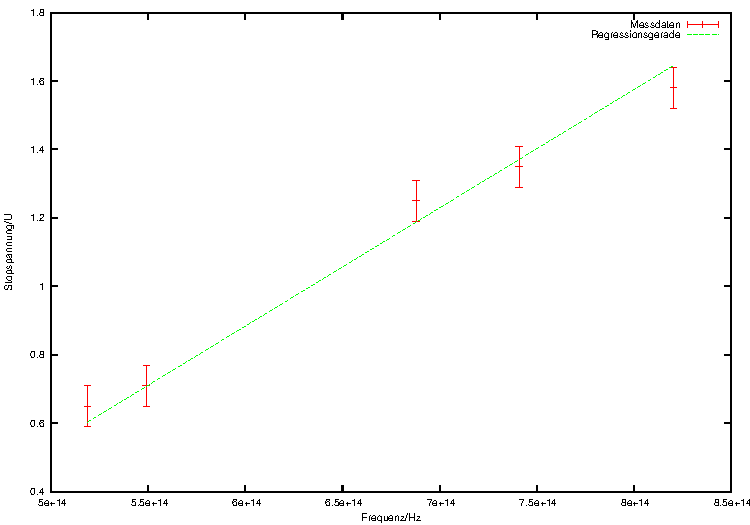
\includegraphics[scale = 1]{a_1_1.pdf}
  	\caption[Plot der Stoppspannung, in Abhängigkeit der Frequenz]{Plot der Stoppspannung, in Abhängigkeit der Frequenz}
  \label{fig:a_3_A}
\end{figure}

Die Regressionsgerade ergab U($\nu$)=(34,6 $\pm 2,4)\cdot10^{-16} \nu$-(1,19 $\pm 0,16)$, das reduzierte $\chi^2$ ergab sich mit 1,00175.

\newpage
Für die 2. Ordnung ergab sich der folgende Plot (Werte aus Tabelle \ref{tab:a_1_2}).

\begin{figure}[H]
\centering
    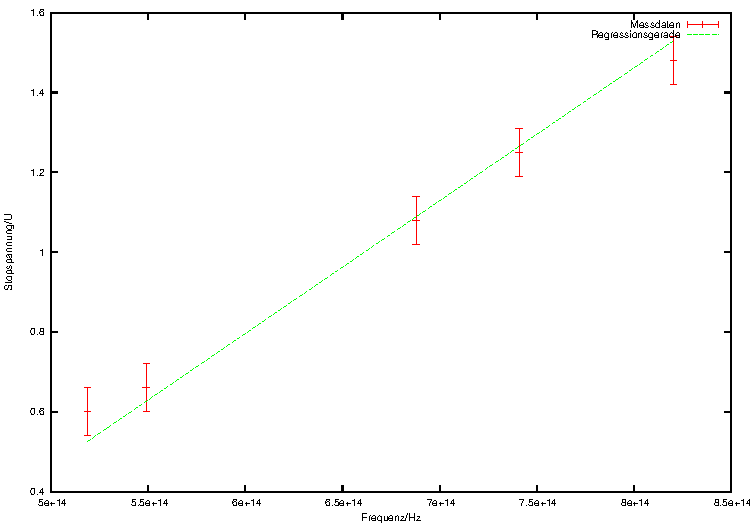
\includegraphics[scale = 1]{a_1_2.pdf}
  	\caption[Plot der Stoppspannung, in Abhängigkeit der Frequenz]{Plot der Stoppspannung, in Abhängigkeit der Frequenz}
  \label{fig:a_3_A}
\end{figure}

Die Regressionsgerade ergab sich mit U($\nu$)=(33,3 $\pm 2,2)\cdot10^{-16} \nu$-(1,2 $\pm 0,1)$, das reduzierte $\chi^2$ ergab sich mit 0.865638.

Aus der Steigung und dem y-Achsenabschnitt der Regressionsgerade sollten das Plancksche Wirkungsquantum und die Austrittsarbeit bestimmt werden. Für die Messungen der 1. Ordnung wurde das Plancksche Wirkungsquantum mit (5,5 $\pm 0,4)\cdot10^{-34}$ Js und die Austrittsarbeit mit (1,9 $\pm 0,3)\cdot10^{-19}$ J. Für die Messung der 2. Ordnung wurde h mit (5,3 $\pm 0,4)\cdot10^{-34}$ Js und die Austrittsarbeit mit (1,9 $\pm 0,2)\cdot10^{-19}$ bestimmt.

Zum Schluss der Messung wurde noch die Abhängigkeit der Stoppspannung von der Intensität gemessen. Dazu wurde ein 20\%, 40\%, 60\%, 80\% und 100\% durchlässiger Intensitätsfilter  verwendet. Die Messdaten finden sich in Tabelle \ref{tab:intänsität}. Die abfallende Stoppspannung entsteht offensichtlich durch Leckströme unseres h/e-Geräts (der 'Kondensator' entlädt sich schneller, als der Aufladevorgang durch den Photostrom).

\subsection{Diskussion}
Das Plancksche Wirkungsquantum hat einen Literaturwert von 6,6$\cdot 10^{-34}$ Js\footnote{Entnommen von http://de.wikipedia.org/wiki/Plancksches\_Wirkungsquantum am  18.09.2014 um 16:15 Uhr}, unserer Wert für die Messung der 1. Ordnung weicht um 16,6\% ab. Der Wert aus der Messung der 2. Ordnung weicht um 19,7\% ab. Diese große  Abweichung erklärt sich über die großen Leckströme, wodurch die von uns gemessene Spannung nicht die echte Stoppspannung ist und wir eine zu geringe Spannung gemessen haben. Der lineare Zusammenhang wird von dem Messdaten bestätigt, dies ist an den Werten der $\chi^2$ zu erkennen. Durch die großen Leckströme erhalten wir auch bei der Messung der Stoppspannung in Abhängigkeit der Intensität kleinere Spannungen, bei geringerer Intensität.

\section{Abschätzung des Photostroms; Quantenausbeute der Photozelle und Lichtleistung}
\subsection{1. Kondensatorkapazität und Photostrom}
\subsubsection{Praktische Durchführung}
Die Photozelle und der Eingang des Meßverstärkers im h/e-Apparat bilden einen kleinen Kondensator, der durch den Photostrom aufgeladen und durch Leckströme im Meßverstärker entladen wird.
Wir wollen aus der Halbwertszeit für den Auf- und Entladevorgang, sowie der Stoppspannung $U_0$ die Kondensatorkapazität und den Photostrom abschätzen. Die Entladekurven haben wir mit einem Oszilloskop vermessen, da unsere Leckströme sehr groß waren.
\subsubsection{Verwendete Formeln}
\textbf{Verwendete Bezeichnungen:}
\begin{enumerate}
\item $I_{photo}$ := Photostrom\\
(Oder Photoelektronenstrom --> hiermit ist ein elektrischer Strom gemeint.)
\item $U_0$ := Stoppspannung
\item $R$ := 'Aufladewiderstand'\\
(Modellhaft wird der Kondensator über einen Widerstand aufgeladen, trivialerweise ergibt sich der verwendete Zusammenhang aus der zugehörigen Differentialgleichung)
\item $t_{1/2_a}$ := Halbwertszeit des Aufladevorgangs
\item $C_{\frac{h}{e}}$ := Kapazität des $\frac{h}{e}$-Gerätes
\item $t_{1/2_e}$ := Halbwertszeit des Entladevorgangs
\item $R_i$ := Innenwiderstand des $\frac{h}{e}$-Gerätes\\
(Der Widerstand charakterisiert die auftretenden Leckströme im $\frac{h}{e}$-Gerät. Er wurde in der Versuchsanleitung mit ca. 10$^{13}\Omega$ geschätzt.)
\end{enumerate}
\textbf{Aus den beiden Halbwertszeiten für den Auf- und Entladevorgang und der Stoppspannung bestimmen wir den Photostrom nach der folgenden Formel:}
\begin{align}
I_{photo} = \frac{U_0}{R}
\label{eqn:i_ph}
\end{align}
Dazu muss einerseits der 'Aufladewiderstand'
\begin{align}
R = \frac{t_{1/2_a}}{\ln(2)C_{\frac{h}{e}}}
\label{eqn:R}
\end{align}
und andererseits die Kapazität unseres $\frac{h}{e}$-Gerätes bestimmt werden.
\begin{align}
C_{\frac{h}{e}} = \frac{t_{1/2_e}}{\ln(2)R_i}
\label{eqn:C}
\end{align}
Die Fehler berechnen sich nach den folgenden Formeln:
\begin{align}
\delta_{I_{photo}}= \sqrt{
\left(\frac{\delta_{U_0}}{R}\right)^2+
\left(\frac{U_0}{R^2}\delta_R\right)^2}
\label{eqn:i_ph_delta}
\end{align}
\begin{align}
\delta_{R}= \sqrt{
\left(\frac{\delta_{t_{1/2_a}}}{\ln(2)C_{\frac{h}{e}}}\right)^2+
\left(\frac{t_{1/2_a}}{\ln(2)C_{\frac{h}{e}}^2}\delta_{C_{\frac{h}{e}}}\right)^2}
\label{eqn:r_delta}
\end{align}
\begin{align}
\delta_{C_{\frac{h}{e}}}= \sqrt{
\left(\frac{\delta_{t_{1/2_e}}}{\ln(2)R_i}\right)^2+
\left(\frac{t_{1/2_e}}{\ln(2)R_i^2}\delta_{R_i}\right)^2}
\label{eqn:c_delta}
\end{align}
\subsubsection{Messergebnisse}
\begin{table}[H]
\caption{Messung zur Bestimmung des Photostroms}
\begin{center}
\begin{tabular}{|l|l|}
\hline
Aufladen &  \\ \hline
t/ms & Fehler/ms \\ \hline
\multicolumn{1}{|r|}{0,36} & \multicolumn{1}{r|}{0,01} \\ \hline
Stoppspannung/V & Fehler/V \\ \hline
\multicolumn{1}{|r|}{1,42} & \multicolumn{1}{r|}{0,06} \\ \hline
Entladen &  \\ \hline
t/ms & Fehler/ms \\ \hline
\multicolumn{1}{|r|}{0,09} & \multicolumn{1}{r|}{0,01} \\ \hline
\end{tabular}
\end{center}
\label{tab:a_2.1}
\end{table}


\subsubsection{Auswertung}
Zur Bestimmung des Photostroms wurde der Widerstand benötigt, dieser wurde über die Kapazität, welche nach Gleichung \ref{eqn:C} und der Fehler nach Gleichung \ref{eqn:c_delta} errechnet wurde. Der Widerstand wurde dann nach Gleichung \ref{eqn:R} und der Fehler nach Gleichung \ref{eqn:r_delta} bestimmt. Daraus wurde nach Gleichung \ref{eqn:i_ph} der Photostrom berechnet und der Fehler mit Gleichung \ref{eqn:i_ph_delta} bestimmt. Für die Kapazität ergab sich ein Wert von (1,30$\pm 0,05)\cdot10^{-14}$F, für den 'Aufladewiderstand' ergab sich ein Wert von (4,0$\pm 0,2)\cdot10^{14}$ $\Omega$. Daraus wurde ein Photostrom vom (3,6$\pm 0,2)\cdot10^{-14}$ A berechnet.

\subsubsection{Diskussion}
Da wir sehr große Leckströme vermuten und unser Gerät sehr alt zu sein schien, ist der in der Versuchsanleitung angegebene Widerstand  mittlerweile warscheinlich viel kleiner. Der daraus errechnete Photostrom sollte deshalb nur die Größenordnung, in der wir uns befinden, angeben. Trotzdem ist der bestimmte Wert sehr klein, was wir uns nur durch die bereits angesprochenen Leckströme sowie den mittlerweile veralteten Wert für den Widerstand des $\frac{h}{e}$-Gerätes erklären können. Durch zu große Leckströme verursachte Messfehler wurden bereits im 4. Teil der 1. Aufgabe angesprochen.


\subsection{2. Die Photozelle als Spektrometer}
\subsubsection{Praktische Durchführung}
Es stehen uns verschiedene Leuchtdioden zur Verfügung. Diese schließen wir an ein Netzgerät an.
(Strom etwa 20 mA, wird durch einen Widerstand bzw. Regler im Anschlussstecker begrenzt)
Wir befestigen die Leuchtdioden nacheinander in der 5-mm-Bohrung einer Kunststoffhalterung und schieben die Halterung waagerecht so über den weißen Schirm des h/e-Apparates, dass das Licht auf die Photozelle gelangen kann. Wir bestimmen dann die jeweiligen Stoppspannungen.
Mit den Ergebnissen aus Versuchsteil 1 können wir, durch Messung der Stoppspannung, die Wellenlänge des Lichtes bestimmen. Diese vergleichen wir mit den Wellenlängen, welche in den Datenblättern der Leuchtdioden angegeben sind. (siehe auch Beschriftung an den Leuchtdioden):
rot = 645 nm, gelb = 583 nm, grün = 565 nm, blau = 470 nm.
%Erklären Sie die Abweichungen zum Literaturwert.
\subsubsection{Verwendete Formeln}
\textbf{Verwendete Bezeichnungen:}
\begin{enumerate}
\item $\lambda$ := Wellenlänge des Lichtes
\item $c$ := Lichtgeschwindigkeit\\
(Verwendet wurde der Literaturwert)
\item $h$ := Plancksches WQ\\
(Verwendet wurde der in Aufgabe 1 bestimmte Wert)
\item $U_0$ := gemessene Stoppspannung\\
(Für jede Diode wird die Stoppspannung wie in Aufgabe 1 gemessen)
\end{enumerate}
\textbf{Die Wellenlängen berechnen wir nach der folgenden Formel, welche sich aus der Einsteinschen Gleichung ergibt:}
\begin{align}
\lambda = \frac{c \cdot h}{U_0\cdot e + W_0}
\label{eqn:lambda}
\end{align}
Der Fehler ergibt sich nach der Formel:
\begin{align}
\delta_{\lambda} = \sqrt{
\left(\frac{c \cdot\delta_h}{U_0\cdot e + W_0}\right)^2+
\left(\frac{c \cdot h \cdot e}{(U_0\cdot e + W_0)^2}\delta_{U_0}\right)^2+
\left(\frac{c \cdot h}{(U_0\cdot e + W_0)^2}\delta_{W_0}\right)^2}
\label{eqn:lambda_delta}
\end{align}


\subsubsection{Messergebnisse}
\begin{table}[H]
\caption{Messung zur Bestimmung der Wellenlängen, der Fehler der Stoppspannung wurde mit 0,06V angenommen}
\begin{center}
\begin{tabular}{|l|r|r|}
\hline
Farbe & \multicolumn{1}{l|}{Stoppspannung/V} \\ \hline
Rot & 0,55 \\ \hline
Gelb & 0,64 \\ \hline
Grün & 1,06 \\ \hline
Blau & 1,39 \\ \hline
\end{tabular}
\end{center}
\label{tab:a_2.2}
\end{table}

\subsubsection{Auswertung}
Es wurden die Wellenlängen für rotes, gelbes, grünes und blaues Licht bestimmt, dafür wurde Gleichung \ref{eqn:lambda} und für den Fehler Gleichung \ref{eqn:lambda_delta} verwendet. Dabei wurde die Lichtgeschwindigkeit mit 299792,458 (km/s) angenommen. Für rotes Licht ergab sich eine Wellenlänge von 596 $\pm$71 nm, für gelbes Licht 566 $\pm$65 nm, für grünes Licht 461 $\pm$47 nm und für blaues Licht 402 $\pm$38 nm.

\subsubsection{Diskussion}
Für rotes Licht wurde ein Wert von 645nm erwartet, was eine Abweichung von 7,6\% ergibt, für gelbes Licht 583nm weicht der von uns bestimmte Wert um  2,9\% ab, bei grünem Licht 565nm weicht unser Wert um 18,4\% ab und bei blauem Licht 470nm weicht der bestimmte Wert um 14,5\% ab. Die Abweichungen erklären sich wieder über große Leckströme, da wir die Daten aus Aufgabe 1 zur Bestimmung verwendet wurde, welche schon eine große Abweichung haben.

\subsection{3. Quantenausbeute der Photozelle und Lichtleistung}
\subsubsection{Praktische Durchführung}
Nicht jedes erzeugte Photoelektron gelangt zur Anode, wenn -- wie in unserem Versuchsaufbau -- die
Photozelle ohne hohe Vorspannung betrieben wird. Die Zahl der im Photostrom nachgewiesenen Photoelektronen ist viel kleiner als die Anzahl der einfallenden Lichtquanten. %(warum?)
Wir wollen das Verhältnis zwischen der Anzahl $N_{ph}$ der Photonen (Lichtquanten), die von der Lichtquelle ausgehend in die Photozelle einfallen, zur
Anzahl $N_{e,Zelle}$ der Elektronen, die von diesen Photonen in der Photozelle produziert werden und den Photostrom bewirken, abschätzen, also: Quantenausbeute = $\frac{N_{e,Zelle}}{N_{ph}}$.
Dazu verwenden wir folgendes Verfahren: Für diese Messung steht uns eine Halbleiter-Photodiode zur Verfügung. Eine solche Photodiode besteht aus einem kleinen Halbleiterkristall. Fällt Licht auf die strahlungsempfindliche Fläche (hier 2, 75 $\times$ 2, 75 mm groß), so werden durch den inneren Photoeffekt Ladungsträger erzeugt, es fließt ebenfalls ein Photostrom. In der Photodiode erzeugt fast jedes einfallende Photon ein Elektron: bei einer Wellenlänge von 850 nm werden
etwa 88 Elektronen pro 100 Lichtquanten erzeugt, für andere Wellenlängen ist das Verhältnis geringer.
Die folgende Abbildung zeigt die Abhängigkeit der relativen spektralen Empfindlichkeit für unseren Photodioden-
typ BPW34 (100 \% entsprechen 88 Elektronen pro 100 Quanten).
%bitte abbildung für die relative empfindlichkeit der photodiode einfügen
\begin{figure}[htbp] 
  \centering
    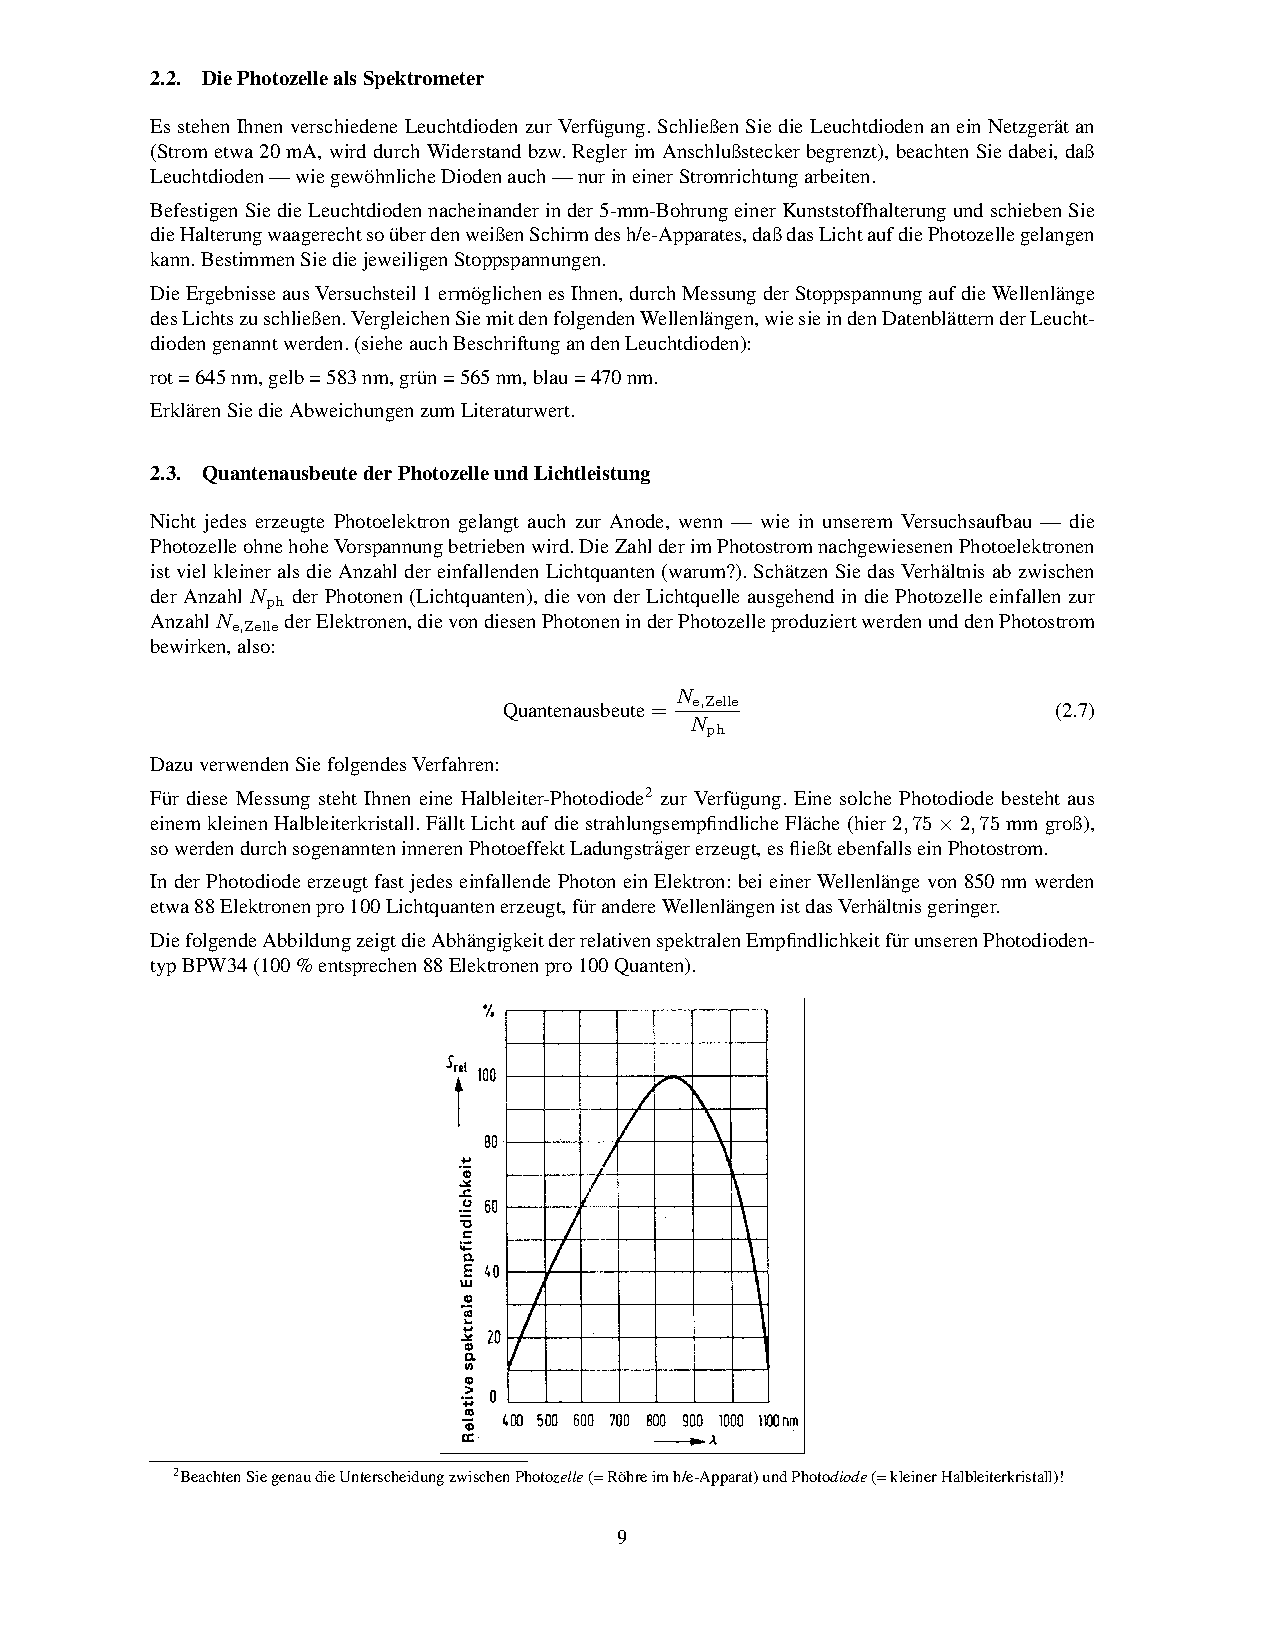
\includegraphics[trim = 35mm 33mm 1mm 170mm, clip, scale = 1]{abb_rel.pdf}
  	\caption[Graphische Darstellung der relativen Empfindlichkeit der Photodiode in Abhängigkeit der Wellenlänge]{Graphische Darstellung der relativen Empfindlichkeit der Photodiode in Abhängigkeit der Wellenlänge\footnotemark}
  \label{fig:schaltskizze}
\end{figure}
\footnotetext{Abbildung entnommen von http://www.atlas.uni-wuppertal.de/~kind/ap22ap2.pdff Seite 9 am 17.09.2014}

Wir schließen die Photodiode an ein Digitalmultimeter an, Messbereich 200 $\mu$A. Die Polarität ist nicht wichtig. Wir halten die Photodiode in den Strahlengang, sodass das Licht einer Spektrallinie auf die Photodiode fällt. Es ist zu beachten, dass die Photodiode etwa den gleichen Abstand von der Lichtquelle hat wie die Photozelle.
%(warum?)
Wir Klappen daher das Lichtschutzrohr zur Seite
und halten die Photodiode vor der Photozelle in das Licht der Spektrallinie.
Wir messen den Photostrom für diese und die anderen Spektrallinien.
Wir können jetzt vom Photostrom der Photodiode auf die Zahl der Elektronen und daraus -- je nach Wellenlänge -- auf die Anzahl der Photonen (pro Zeitintervall) schließen. Wir nehmen an, dass die Öffnung an der Photozelle etwa so groß ist wie die Fläche der Photodiode, d.h. beide erhalten etwa gleich viel Photonen — vorausgesetzt, beide haben den gleichen Abstand zur Lichtquelle. Den Photostrom der Photozelle haben wir in Teil 1 abgeschätzt. Hiermit bestimmen wir die Quantenausbeute der Photozelle. Zuerst bestimmen wir die Anzahl der Photonen (pro Zeitintervall), aus der Wellenlänge und der Planckschen Konstanten können wir dann die Energie jedes Photons berechnen. Wir bestimmen die Lichtleistung, die mit den einzelnen Spektrallinien auf die Photozelle gelangt.

\subsubsection{Verwendete Formeln}
\textbf{Verwendete Bezeichnungen:}
\begin{enumerate}
\item $I_k$ := Photoelektronenstrom\\
(Der Strom der Photoelektronen wird aus dem Diagramm in der Versuchsanleitung sowie mit dem an der \textbf{Photodiode} gemessenen Photostrom bestimmt. Den Photonenstrom, also die Anzahl der Photonen pro Zeitintervall erhält man nach teilen durch die Elementarladung.)
\item $I_{Diode}$ := gemessener Diodenstrom\\
(bzw. Photostrom der \textbf{Photodiode})
\item $\Gamma(\lambda)$ := Korrekturfaktor\\
(Wird am Graph für die relative Empfindlichkeit der Photodiode abhängig von der Wellenlänge abgelesen.)
\item $\frac{N_{e,Zelle}}{N_{ph}}$ := Quantenausbeute
\item $I_{photo}$ := Photostrom\\
(Oder Photoelektronenstrom --> hiermit ist ein elektrischer Strom gemeint. Dies ist der für die \textbf{Photozelle} in Aufgabe 2.1 bestimmte Wert für den Photostrom!)
\item $P_{Licht}$ := Lichtleistung
\item $h$ := Plancksches WQ
(In diesem Aufgabenteil wurde der Literaturwert für h benutzt. Der Fehler kann deshalb vernachlässigt werden.)
\item $f$ := Frequenz der Lichtes
(Aus der Versuchanleitung und ohne Fehler angenommen)
\item $e$ := Elementarladung
(Literaturwert)
\end{enumerate}
\textbf{Der Photoelektronenstrom bestimmt sich durch die Formel:}
\begin{align}
I_k = \frac{I_{Diode}}{0,88*\Gamma(\lambda)}
\label{eqn:i_k}
\end{align}
Mit dem Fehler:
\begin{align}
\delta_{I_k} = \sqrt{
\left(\frac{\delta_{I_{Diode}}}{0,88*\Gamma(\lambda)}\right)^2+
\left(\frac{I_{Diode}}{0,88*(\Gamma(\lambda))^2}
\delta_{\Gamma(\lambda)}\right)^2}
\label{eqn:i_k_delta}
\end{align}
\textbf{Die Quantenausbeute berechnet sich durch:}
\begin{align}
\frac{N_{e,Zelle}}{N_{ph}} = \frac{I_{photo}}{I_{k}}
\end{align}
Mit einem Fehler von:
\begin{align}
\delta_{\frac{N_{e,Zelle}}{N_{ph}}} = \sqrt{
\left(\frac{\delta_{I_{photo}}}{I_{k}}\right)^2+
\left(\frac{I_{photo}}{I_{k}^2}\delta_{I_{k}}\right)^2}
\end{align}
\textbf{Die Lichtleistung berechnen wir mit der Formel:}
\begin{align}
P_{Licht} = \frac{h\cdot f\cdot I_k}{e}
\label{eqn:p_l}
\end{align}
Mit einem Fehler von:
\begin{align}
\delta_{P_{Licht}} = \frac{h\cdot f\cdot \delta_{I_k}}{e}
\label{eqn:p_l_delta}
\end{align}

\subsubsection{Messergebnisse}
\begin{table}[H]
\caption{Messung des Strom in der Photodiode, zur Bestimmung der Quantenausbeute und der Lichtleistung.}
\begin{center}
\begin{tabular}{|l|r|r|}
\hline
Farbe & \multicolumn{1}{l|}{Strom/$\mu$A} & \multicolumn{1}{l|}{Fehler/$\mu$A} \\ \hline
Ultraviolett & 0,06 & 0,01 \\ \hline
Violett & 0,07 & 0,01 \\ \hline
Blau & 0,09 & 0,01 \\ \hline
Grün & 0,08 & 0,01 \\ \hline
Gelb & 0,11 & 0,01 \\ \hline
\end{tabular}
\end{center}
\label{tab:a_2.3}
\end{table}

\begin{table}[H]
\caption{Aus dem Graphen abgelesene Korrekturwerte $\Gamma(\lambda)$}
\begin{center}
\begin{tabular}{|l|r|}
\hline
Farbe & \multicolumn{1}{l|}{Zusätzlicher Korrekturfaktor in \%} \\ \hline
Ultraviolett & 7 \\ \hline
Violett & 11 \\ \hline
Blau & 27 \\ \hline
Grün & 43 \\ \hline
Gelb & 54 \\ \hline
\end{tabular}
\end{center}
\label{tab:a_2_3_k}
\end{table}


\begin{table}[H]
\caption{Photoelekronenstrom der verschiedenen Farben, Werte bestimmt nach Gleichung \ref{eqn:i_k} und der Fehler nach Gleichung \ref{eqn:i_k_delta}}
\begin{center}
\begin{tabular}{|l|r|r|}
\hline
Farbe & \multicolumn{1}{l|}{I\_k/A} & \multicolumn{1}{l|}{Fehler/A} \\ \hline
Ultraviolett & 6,5E-007 & 2E-007 \\ \hline
Violett & 6,2E-007 & 1E-007 \\ \hline
Blau & 5,1E-007 & 0,4E-008 \\ \hline
Grün & 4,2E-007 & 0,3E-008 \\ \hline
Gelb & 6,9E-007 & 0,2E-008 \\ \hline
\end{tabular}
\end{center}
\label{tab:i_k}
\end{table}

\begin{table}[H]
\caption{Anzahl der Photonen pro Zeiteinheit.}
\begin{center}
\begin{tabular}{|r|r|}
\hline
\multicolumn{1}{|l|}{Anzahl Photonen pro Sekunde/(1/s)} & \multicolumn{1}{l|}{Fehler/(1/s)} \\ \hline
4E012 & 1E012 \\ \hline
3,9E012 & 0,6E012 \\ \hline
3,2E012 & 0,3E012 \\ \hline
2,6E012 & 0,2E012 \\ \hline
4,3E012 & 0,1E012 \\ \hline
\end{tabular}
\end{center}
\label{tab:a_2_3_a}
\end{table}

\begin{table}[htbp]
\caption{Quantenausbeute für die verschiedenen Farben}
\centering
\begin{tabular}{|l|r|r|}
\hline
Farbe & \multicolumn{1}{l|}{Ausbeute} & \multicolumn{1}{l|}{Fehler} \\ \hline
Ultraviolett & 6E-008 & 1E-008 \\ \hline
Violett & 6E-008 & 1E-008 \\ \hline
Blau & 7,0E-008 & 0,7E-008 \\ \hline
Grün & 8,4E-008 & 0,7E-008 \\ \hline
Gelb & 5,1E-008 & 0,3E-008 \\ \hline
\end{tabular}
\label{tab:ausbeute}
\end{table}


\subsubsection{Auswertung}
In der letzten Aufgabe sollte die Quantenausbeute sowie die Lichtleistung bestimmt werden. Dazu wurde der mit der Photodiode gemessene Strom zuerst mit dem Korrekturfaktor $\frac{1}{0,88}$ multipliziert und dann mit den jeweiligen spezifischen Korrekturfaktoren aus dem Graph in der Versuchsdurchführung (bzw. in der Versuchsanleitung) multipliziert (Tabelle \ref{tab:a_2_3_k}). Die dabei bestimmten Quantenausbeute ergibt das folgende Diagramm.

\begin{figure}[H]
\centering
    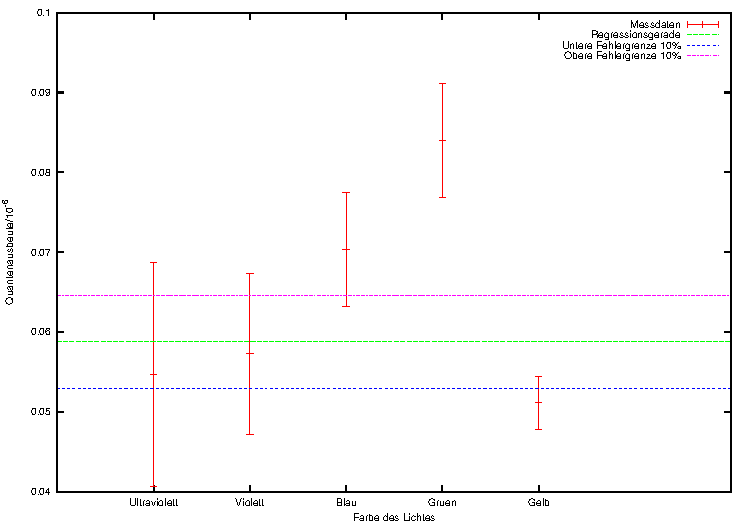
\includegraphics[scale = 1]{a_2_2.pdf}
  	\caption[Graphische Darstellung der Quantenausbeute für die verschiedenen Wellenlängen]{Graphische Darstellung der Quantenausbeute für die verschiedenen Wellenlängen}
  \label{fig:a_2_3}
\end{figure}

Die Messwerte wurden mit einer Konstanten gefittet, dabei ergab sich ein Wert von (0,059$\pm 0,006)\cdot10^{-6}$ mit einem reduzierten $\chi^2$ von ca. 5,12. Nach Gleichung \ref{eqn:p_l} wurde die Lichtleistung berechnet und der Fehler nach Gleichung \ref{eqn:p_l_delta}, es ergeben sich die folgende Werte.

\begin{table}[H]
\caption{Berechnete Lichtleistungen}
\begin{center}
\begin{tabular}{|l|r|r|}
\hline
Farbe & \multicolumn{1}{l|}{Leistung/W} & \multicolumn{1}{l|}{Fehler/W} \\ \hline
Ultraviolett & 1,4E-007 & 0,3E-007 \\ \hline
Violett & 1,8E-007 & 0,3E-007 \\ \hline
Blau & 3,4E-007 & 0,3E-007 \\ \hline
Grün & 3,6E-007 & 0,2E-007 \\ \hline
Gelb & 7,1E-007 & 0,2E-007 \\ \hline
\end{tabular}
\end{center}
\label{tab:a_2_3_l}
\end{table}


\subsubsection{Diskussion}
Da wir keine Referenzwerte haben, können wir keine Aussage unsere Messergebnisse treffen. Durch die bereits angesprochenen systematischen Fehler ist zu erwarten, dass die Quantenausbeute ebenfalls einen großen Fehler hat.

\section{Fazit}
Alle Messergebnisse, die wir mit Literaturwerten vergleichen konnten, weisen eine große Abweichung auf, wir vermuten große Leckströme in unserem $\frac{\text{h}}{\text{e}}$-Gerät. Insgesamt konnten wir konsistente Messergebnisse erzielen, wobei sich der systematische Fehler aus der ersten Aufgabe auf die daraus berechneten Größen in der zweiten Aufgabe auswirkt. Im ersten Teil der zweiten Aufgabe vermuten wir eine fehlerhafte Angabe des Widerstandes für das $\frac{\text{h}}{\text{e}}$-Gerät, welcher aus der Versuchsbeschreibung entnommen wurde. Dadurch ergeben sich im dritten Aufgabenteil der zweiten Aufgabe, schlechte Werte für die Quantenausbeute.

 %Werte stimmen mit den Formeln überein/nicht überein 
 %
\end{document}

